\documentclass[12pt]{article}
    % \usepackage{polski}
    \usepackage[utf8]{inputenc}
    
    \usepackage{lingmacros}
    \usepackage{tree-dvips}
    \usepackage{blindtext}
    \usepackage{graphicx}
    \usepackage{todonotes}
    \usepackage{amsmath}
    \usepackage{ amssymb }    
    \usepackage{hyperref}    
    
    \graphicspath{ {imgs/} }
    
    \newcommand{\norm}[1]{\left\lVert#1\right\rVert}    
    
    \setcounter{secnumdepth}{0}
    % \pagenumbering{gobble}
    
    % \usepackage[top=0.1in, bottom=0.7in, left=1.35in, right=1.35in]{geometry}
    
    \title{Lifelong Learning With Dynamically Expandable Networks -- Reproducibility Report }
    \author{Błażej Sowa, Łukasz Siudek}
    \date{}
    
    \begin{document}
    \maketitle
    
    \section {Motivation}

    Reproducibility of results in machine learning is crucial in order to make the experiment believable.
    However, many researchers state that there exists a reproducibility crisis on the science field.
    This problem seems to concern engineering studies, and among others -- machine
    learning. This might be a major problem, cosidering the fact that machine learning is a very fast
    growing field of research.
    To make projects reproducible, several points have to be taken into consideration, some of which are
    listed in this report.
    
    \section{Introduction}
    
    In this report we are going to show our results of attempted reproduction of a
    recent conference paper from ICLR, called "Lifelong Learning With Dynamically
    Expandable Networks" which proposes a novel deep neural network for lifelong learning, called "Dynamically
    Expandable Network". It performs partial retraining of the network trained on old tasks by exploiting task
    relatedness, while increasing its capacity when necessary to account for new knowledge required
    to account for new tasks, to find the optimal capacity for itself, while also effectively preventing
    semantic drift.
    
    \section {Reproducibility}
    
    \subsection {Available Information Overview}
    
    In this section, we list important reproducibility metrics.  
    
    \subsubsection{Dataset}
    % Information about the location and the retrieval process of the dataset is needed to
    % ensure access to the dataset as used in the study.
    We use the same datasets as those introduced in the paper.
    \begin{enumerate}  
        \item CIFAR-10
        \item MNIST-Variation 
    \end{enumerate}
    
    \subsubsection{Data preprocessing}
    % The process of ridding the input data of noise and encoding it into a
    % format acceptable to the learning algorithm. Explicit preprocessing information is the first
    % step towards a successful reproduction exercise. An independent researcher should be able
    % to follow and repeat how the data was preprocessed in the study. Also, it will be useful to
    % find preprocessing output information to compare to e.g. final feature vector dimension
    Authors of the paper say, that in the MNIST-Variation the handwritten digits are rotated to
    arbitrary angles and have noise in the background, which makes the prediction task more challenging.
    \\
    \\
    We use the same preprocessing methods on the MNIST dataset. At first, we aplly random rotation
    to the images. Then, we add Gaussian noise with our custom parameters $\mu = 0$ and $\sigma = 0.2$.
    
    \subsubsection{Dataset Partitions}
    %  Details of how the dataset was divided for use as training and test data.
    For the MNIST dataset, the authors of DEN paper use 1,000/200/5,000 images for
    train/val/test split for each class.
    They form each task to be one-versus-rest binary classification.
    \\
    \\
    For the CIFAR-10 dataset, for each class, $5,000$ out of $6,000$ images are used for training and the remainder
    is used for test.
    
    \subsubsection{Model training}
    % The process of fitting the model to the data. Making available, as much
    % information as possible regarding every decision made during this process is particularly
    % crucial to reproduction. Necessary information include but not limited to:
    % 1. Study parameters
    % 2. Proposed technique details – codes, algorithms etc. (if applicable)
    Out of two specified datasets, the MNIST dataset is trained by Feedforward networks and Convolutional
    neural networks are used in oder to train the CIFAR-10 dataset.
    \\
    \\
    Out of several models introduced in the paper, we have implemented the following Feedforward networks:
    \begin{enumerate}  
        \item DNN-STL. Base deep neural network, each task has its own network and exacltly one output.
        \item DNN-MTL. Base DNN trained for all tasks at once. One network with many outputs.
        \item DNN-L2. Base DNN, where at each task $t$, $W^{t}$ is initialized as $W^{t-1}$ and continously
        trained with SGD, with $l_{2}$-regularization between $W^{t}$ and $W^{t-1}$. For this purpose, we use
        the equation:

        $$ \underset{W_{l}^{\mathcal{N}}}{\text{minimize }} \mathcal{L}(W^{t}; \mathcal{D}_{t}) + \lambda \norm{W^{t} - W^{t-1}}^{2}_{2}, $$

        where $\lambda = 0.005$.

        \item DNN. Same as previous, but no $l_{2}$-regularization is used.
        \item DEN. Dynamically Expandable Network, but only with Selective Training algorithm used.   
    \end{enumerate}
    \bigskip
    We use two-layer network with 312-128 neurons with ReLU activation.
    When it comes to the Convolutional networks, we use LeNet, with two convolutional layers
    and three fully-connected layers.
    \\
    \\
    In model training, we used SGD with momentum $0.9$ and weight decay parameter equal to $10^{-4}$.
    These parameters were not stated in the original paper, so we came up with our own.
    
    % \subsubsection{Model Assessment}
    % Measuring the performance of the model trained in 2. Similar information
    % as in 2 applies here as well.
    
    \subsubsection{Randomization control}
    % Most operations of machine learning algorithms involves randomization.
    % Therefore, it is essential to set seed values to control the randomization process in
    % order to be able to repeat the same process again.
    Authors of the paper do not state how they set seed values. On the other hand, we use constant
    seed value.
    
    \subsubsection{Software and Hardware Environment}
    % Due to the fact that software packages/modules are in continual
    % development with possible alterations to internal implementation algorithms, it is important
    % that the details of the software environment used (modules, packages and version numbers)
    % be made available.
    All models and algorithms in the DEN paper were implemented using the Tensorflow library.
    Package version is not specified.
    \\
    \\
    In order to implement our version of the network, we used PyTorch (version 0.3.0.post4).
    \\
    \\
    Our hardware setup (GCloud virtual machine):
    \begin{itemize}
        \item 4 x vCPU
        \item 16GB RAM
        \item NVIDIA Tesla K80
    \end{itemize}
    \bigskip
    No hardware information is given about the machine used in the DEN paper.

    % Some data intensive studies are only
    % reproducible on the same machine capacity as was used to produce the original result. So,
    % the hardware information are sometimes essential.
    
    \subsection {Results}

    In this section, we are going to show our results and explain encountered issues.

    \subsubsection{Performance evaluation}

    In order to evaluate performance of the networks we had to implement the AUROC (The Area Under an ROC
    Curve) function, where ROC curve is created by plotting the true positive rate against the false
    positive rate at various thresholds. The larger the computed area, the better our binary classification works. 
    \\
    \\
    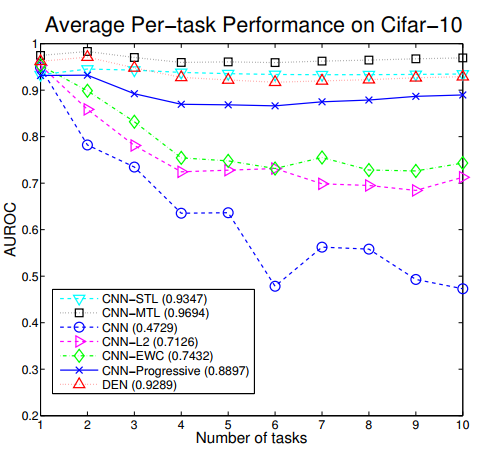
\includegraphics[height=6cm]{paper-cifar-10.png}
    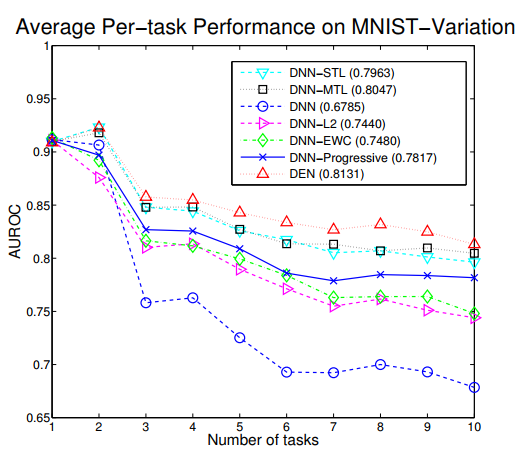
\includegraphics[height=6cm]{paper-mnist-var.png}

    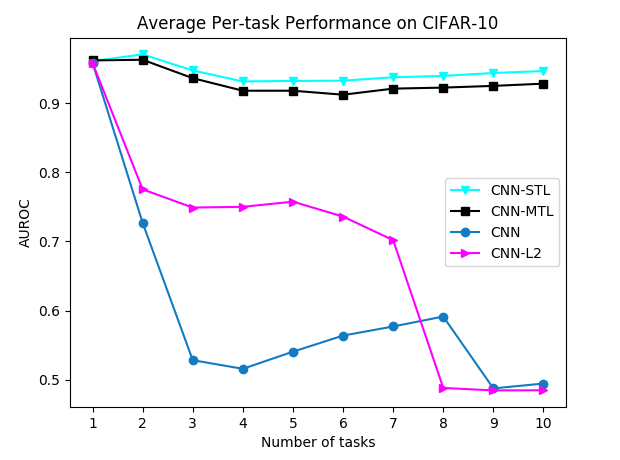
\includegraphics[height=5cm]{fig1-s.png}
    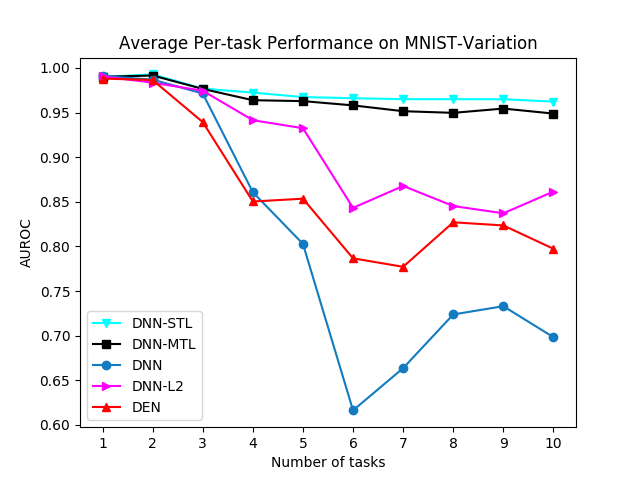
\includegraphics[height=5cm]{fig2-v2.png}

    \section {Conclusion}
    
    Conclusion.

    \section{Acknowledgments}

    The authors thank Google for GCE Credits awarded through Google Cloud Platform Education Grants
    to the Neural Networks and Deep Learning course and to this project.    
        
    \begin{thebibliography}{9}
        \bibitem{den}
            Jaehong Yoon, Eunho Yang, Sung Ju Hwang,
            \textit{Lifelong Learning with Dynamically Expandable Networks},
            arXiv:1708.01547v1.

        \bibitem{lenet}
            Y. Lecun, L. Bottou, Y. Bengio, and P. Haffner,
            \textit{Gradient-based Learning Applied to Document Recognition},
            Proceedings of the IEEE, 86(11):2278–2324, 1998.

        \bibitem{lenet}
            Babatunde K. Olorisade, Pearl Brereton, Peter Andras, 
            \textit{Reproducibility in Machine Learning-Based Studies: An Example of Text Mining},
            16 Jun 2017, ICML 2017 RML Submission.

        \bibitem{crisis}
            Monya Baker,
            \href{https://www.nature.com/news/1-500-scientists-lift-the-lid-on-reproducibility-1.19970}{1,500 scientists lift the lid on reproducibility},
            25 May 2016, corrected 28 July 2016.

    \end{thebibliography}
    
    \end{document}
        